\documentclass[a4paper, usenatbib, 12pt]{article}
\usepackage{subfig}
\usepackage{float}
\usepackage{wrapfig}
\usepackage{graphicx}
\usepackage{amsmath}
\usepackage{amssymb}
\usepackage{booktabs}
\usepackage{cite}
\usepackage[icelandic,spanish,english]{babel}
\usepackage[T1]{fontenc}
\usepackage[utf8]{inputenc}
\usepackage[top=3.5cm, bottom=2.5cm, left=3.5cm,right=3.5cm]{geometry} 

%----------------------New commands -------------------

\newcommand{\tol}{Tololo 1214-277}
\newcommand{\lya}{Ly$\alpha$}
\newcommand{\hb}{H$\beta$}
\newcommand{\ha}{H$\alpha$}
\newcommand{\oiii}{[OIII]}
\newcommand{\oii}{[OII]}
\newcommand{\nii}{[NII]}
\newcommand{\esca}{erg cm$^{-2}$ s$^{-1}$ \AA$^{-1}$}
\newcommand{\esc}{erg cm$^{-2}$ s$^{-1}$}
\newcommand{\es}{erg s$^{-1}$}
\newcommand{\esa}{erg s$^{-1}$}
\newcommand{\kms}{km s$^{-1}$}
\newcommand{\apj}{ApJ}  
\newcommand{\jcap}{JCAP}  
\newcommand{\apjs}{ApJS}  
\newcommand{\pasa}{PASA}  
\newcommand{\apjl}{ApJL}  
\newcommand{\aj}{AJ}  
\newcommand{\mnras}{MNRAS}  
\newcommand{\mnrassub}{MNRAS accepted}  
\newcommand{\aap}{A\&A}  
\newcommand{\aaps}{A\&AS}  
\newcommand{\araa}{ARA\&A}  
\newcommand{\nat}{Nature}  
\newcommand{\physrep}{PhR}
\newcommand{\pasp}{PASP}    
\newcommand{\pasj}{PASJ}    
\newcommand{\sigmaclump}{$69^{+17}_{-15}$ km s$^{-1}$}
\newcommand{\inftyclump}{$79^{+73}_{-42}$ km s$^{-1}$}
\newcommand{\probaclump}{$0.78^{+0.16}_{-0.43}$}
\def\simgt{\lower.5ex\hbox{\gtsima}}
\def\simlt{\lower.5ex\hbox{\ltsima}}
%------------------------------------------------------

\begin{document}
\pagestyle{empty}
\noindent
\textbf{Lyman-$\alpha$ emission sketches a massive dwarf}
\\
\\
Jaime E. Forero-Romero$^{1}$, Max Groenke$^2$, Mar\'ia Camila
Remolina-Guti\'errez$^1$, Juan Nicol\'as
Garavito-Carmargo$^3$, Mark Dijkstra$^2$.
\\
\\
\scriptsize
{$^1$ Departamento de Física, Universidad de los Andes, Cra. 1
  No. 18A-10 Edificio Ip, CP 111711, Bogot\'a, Colombia 
\\
$^2$ Institute of Theoretical Astrophysics, University of Oslo,
Postboks 1029 Blindern, NO-0315 Oslo, Norway.
\\
$^3$ Department of Astronomy, University of Arizona, 933 North Cherry
Avenue, Tucson, AZ 85721, USA. 
\normalsize
\\
\\
\textbf{
  Star-forming Compact Dwarf Galaxies (CDGs) resemble the expected
  pristine conditions of the first galaxies in the Universe.    
Before the observational detection of the first galaxies becomes
reality, CDGs are the best systems to test our ideas on primordial
galaxy formation and evolution.    
Here we report on one of such CDGs, \tol, which presents
a broad symmetric Lyman-$\alpha$ emission that had evaded theoretical
interpretation so far. 
In this letter we explain these features by two different models: an
homogeneous gaseous sphere undergoing bulk rotation and an interstellar
medium composed by outflowing clumps with additional random motions.
It is the first time that an observed \lya\ spectrum can be explained
assuming either of these physical conditions.
We find that both models independently require high velocities
(either a bulk rotation of $348^{+75}_{-48}$ km s$^{-1}$ or a clump velocity
dispersion of \sigmaclump with outflows of
$79^{+73}_{-42}$ km s$^{-1}$) consistent with a dynamical mass at
least $10$ times larger than its baryonic mass.  
We argue that the most plausible explanation for this excess of
dynamical mass is the presence of a supermassive black hole at the
center of \tol. 
This work demonstrates the importance of considering multiphase
physics and rotation among the possible conditions shaping the
\lya\ spectra of the first galaxies.  
Additionally, if future kinematic maps of \tol\ confirm the high
velocities postulated in our model, it would provide new
evidence for dwarf galaxies as hosts of supermassive black
holes.  
}  



The first generation of galaxies trace our cosmic origins. 
They were the first steps in the evolution of galaxies such as the Milky
Way. 
In the standard Big Bang cosmology the only chemical elements that
were created in the nucleosynthesis process were Hydrogen, Helium and
Lithium.  
Heavier elements must have been created in stellar evolution process. 
Therefore, we expect the first generation of
galaxies to be metal free and rich in Hydrogen. 
This kind of primordial galaxies have not been detected yet. 
However, dwarf star forming galaxies with a low metallicity content
are seen as templates to understand the early galaxy evolution process. 

Almost fifty years ago \cite{PartridgePeebles} it was realized that
young galaxies could be detected through a strong Lyman-$\alpha$ line
emission.  
This theoretical prediction was only confirmed thirty year later on
distant, relatively young, not primordial, galaxies.
Currently Lyman Alpha Emitting (LAE) galaxies are commonly targeted
in surveys. 
The presence of the Ly-$\alpha$ emission line provides confirmation of
the distance of a galaxy while provides clues about the stellar
population and inter-stellar medium conditions regulating the
Ly-$\alpha$ emission. 

The Ly-$\alpha$ emission line is not exclusive of distant galaxies. 
Any galaxy with low dust content and ongoing star formation has the
right conditions to show this line.  
There are, for instance,  local Universe surveys that target
Ly-$\alpha$ emission in nearby dwarf star forming galaxies 
\cite{LARS}. 
The study of nearby LAE samples has allowed the study of other
indicators that might be more difficult to obtain for distant galaxies
such as morphology, dust attenuation, neutral hydrogen contents and
ionization state.  

However, the physical interpretation of Ly-$\alpha$ observations is
not straightforward \cite{2015ApJ...805...14R}. 
This is due to the resonant nature of the Ly-$\alpha$ line. 
A Ly-$\alpha$ photon follows a diffusion-like process before escaping
the galaxy or being absorbed by dust. 
The resulting line profile becomes sensitive to the dynamical, chemical
and thermal conditions in the interstellar medium. 
There are very few analytically tools available to interpret the
Ly-$\alpha$ line.
They are applicable only in very few cases of highly symmetrical
conditions, which are hardly met in real astrophysical systems.
For these reasons the interpretation of Ly-$\alpha$ observations
require state-of-the-art Monte Carlo radiative transfer simulations.   


\tol\ is a compact star forming dwarf galaxy that presents a
strong Ly-$\alpha$ emission \cite{Thuan97} with two puzzling 
features: it is symmetric and single peaked.
Commonly, the Ly-$\alpha$ line has a single or asymmetric double peak. 
These two special features in \tol\ cannot be explained with
conventional models \cite{2006A&A...460..397V,2015ApJ...812..123G}.  

In this letter we show how the \tol's \lya\ profile can be explained
either by rotation or the recently developed class of more complex
multiphase models that predict a wider variety of spectra
including, single, double and triply peaked spectra.  
Figure 1. summarizes our findings.
Dots represent the observational data for \tol\ with the
overplot from our best fits from the analytical solution for a
rotating homogeneous gas sphere (continuous line) and the multiphase
model (dashed line). 
This is the first time that these models have been introduced with
success to explain an observed \lya\ profile.   


The best parameters in the rotation model are a rotational velocity of 
$V_{\rm max}=348^{+75}_{-48}$ \kms, an optical depth
$\log_{10}\tau=6.96^{+0.26}_{-0.18}$,  and a temperature of $\log_{10}
T/\mathrm {K} = 4.27^{+0.11}_{-0.18}$.  
This model is also able to constrain the angle between the plane
perpendicular to the rotation axis and the observational line-of-sight
to $\theta = 35.78^{+2.13}_{-1.88}$ degrees.

In the multiphase model the best constrained parameters are
the clump velocity dispersion  $\sigma_{\rm{cl}}=$\sigmaclump\,
the clump's outflowing velocity $v_{\infty, \rm{cl}}=$\inftyclump\
and the fraction of the \lya\ emission that is  coming
from the cold clumps  $P_{\rm cl}=$\probaclump.
The multiphase model assumes that the clouds are distributed over a
sphere of $5$kpc in radius, close to the $\approx 4$kpc physical size
of \tol\ as determined by optical imaging.
The assumed physical size and the velocity dispersion $\sigma_{\rm
  cl}$ correspond to a  dynamical mass of  $M_{\rm
  dyn}=2.8^{+1.3}_{-1.2}\times 10^{9}$ $M_{\odot}$. In the rotation
model assuming reasonable bounds for the number density of neutral Hydrogen atoms (
$0.01<n/\mathrm{atoms\ cm^{-3}}<0.1$) and using $\tau=10^7$ the radius
of the emission region can be bracketed to be in $0.55 <
r_s/\mathrm{kpc}< 5.5$.
Using $V_{\rm max}=300$km s$^{-1}$, we find a dynamical mass range of
$5.45\times 10^{9}M_{\odot} < M_{\rm dyn} < 5.45\times 10^{10} M_{\odot}$.  

Are these values atypical? If \tol\ followed the fundamental
plane relationship between its mean surface brightness
$I_e$, the projected half-light radius $R_e$ and the velocity dispersion
$\sigma$, described by $\log I_e=1.6 \log\sigma - 1.21\log R_e +
0.55$ \cite{2009ApJ...698.1590G},  the expected velocity dispersion
should be on the order of $5 \pm 1$ 
\kms, which is a factor of $\sim$ $12$ - $60$ lower than the 
results from the multiphase and rotation models, respectively. 
These are equivalente to factors of $\sim$ $140$ - $3600$ on the
dynamical mass;
\tol\ seems to be significantly more massive than the expectation from
scaling relationships for dwarf ellipticals.
A factor of $100$ in dynamical mass could be accounted by dark matter if
\tol\ was hosted by a dark matter halo of  $\sim 10^{16}$ M$_{\odot}$
\cite{2011ApJ...726..108T}, which is very unlikely as it would mean that
\tol\ is at the center of a super rich cluster of galaxies,
contradicting observational evidence.
The remaining possibility is that \tol\ hosts a supermassive black hole of
$\sim 5\times 10^{9}$ M$_{\odot}$, corresponding to $10$ times its
estimated stellar and gaseous mass.


A new observational test is needed to clarify the physical nature of
\tol. 
We suggest that integral field unit measurements spatially
resolving its spatial extent is up to the task. 
\tol\ spans a region of $4$ arcseconds,
an instrument such as the Multi Unit Spectroscopic Explorer
\cite{2014Msngr.157...13B} with its
nominal $0.2$ arcseconds spatial sampling over a $1.0$ arcminute field
in wide-field mode could provide a coarse mapping of different
ionization lines to infer a kinematic map.
Another observational test includes the measurement of the escape
fraction of \lya\ continuum ionizing radiation. 
In the rotational model this fraction should be zero, while
the multiphase model predicts that averaging over all sightlines
it should be around $0.5^{+1.0}_{-0.4}$\%, with the possibility of strong
variations depending on viewing angle. 

All in all, the mere existence of a strong LAE galaxy with a broad,
symmetric line is interesting.
It raises the question whether some high redshift LAEs have asymmetric
lines because the blue half was truncated by the intergalactic medium.
In this case the \lya\ radiation could emerge as a low surface
brightness glow, which may be connected to \lya\ halos, while also
influencing the way LAEs can be used as a probe of reionization
\cite{2014PASA...31...40D}.  

These findings demonstrate the importance of including rotation and multiphase
conditions as features to model the \lya\ line in high redshift
galaxies.
Additionally, if the hypothesis of a supermassive black
hole in \tol\ proves to be consistent with future observational
kinematic maps, it could correspond to a so far undetected black hole
in a dwarf galaxy, providing a new way to test and probe
theories on the co-evolution of galaxies and black holes in the first
generation of galaxies.  

\begin{figure}
\begin{center}
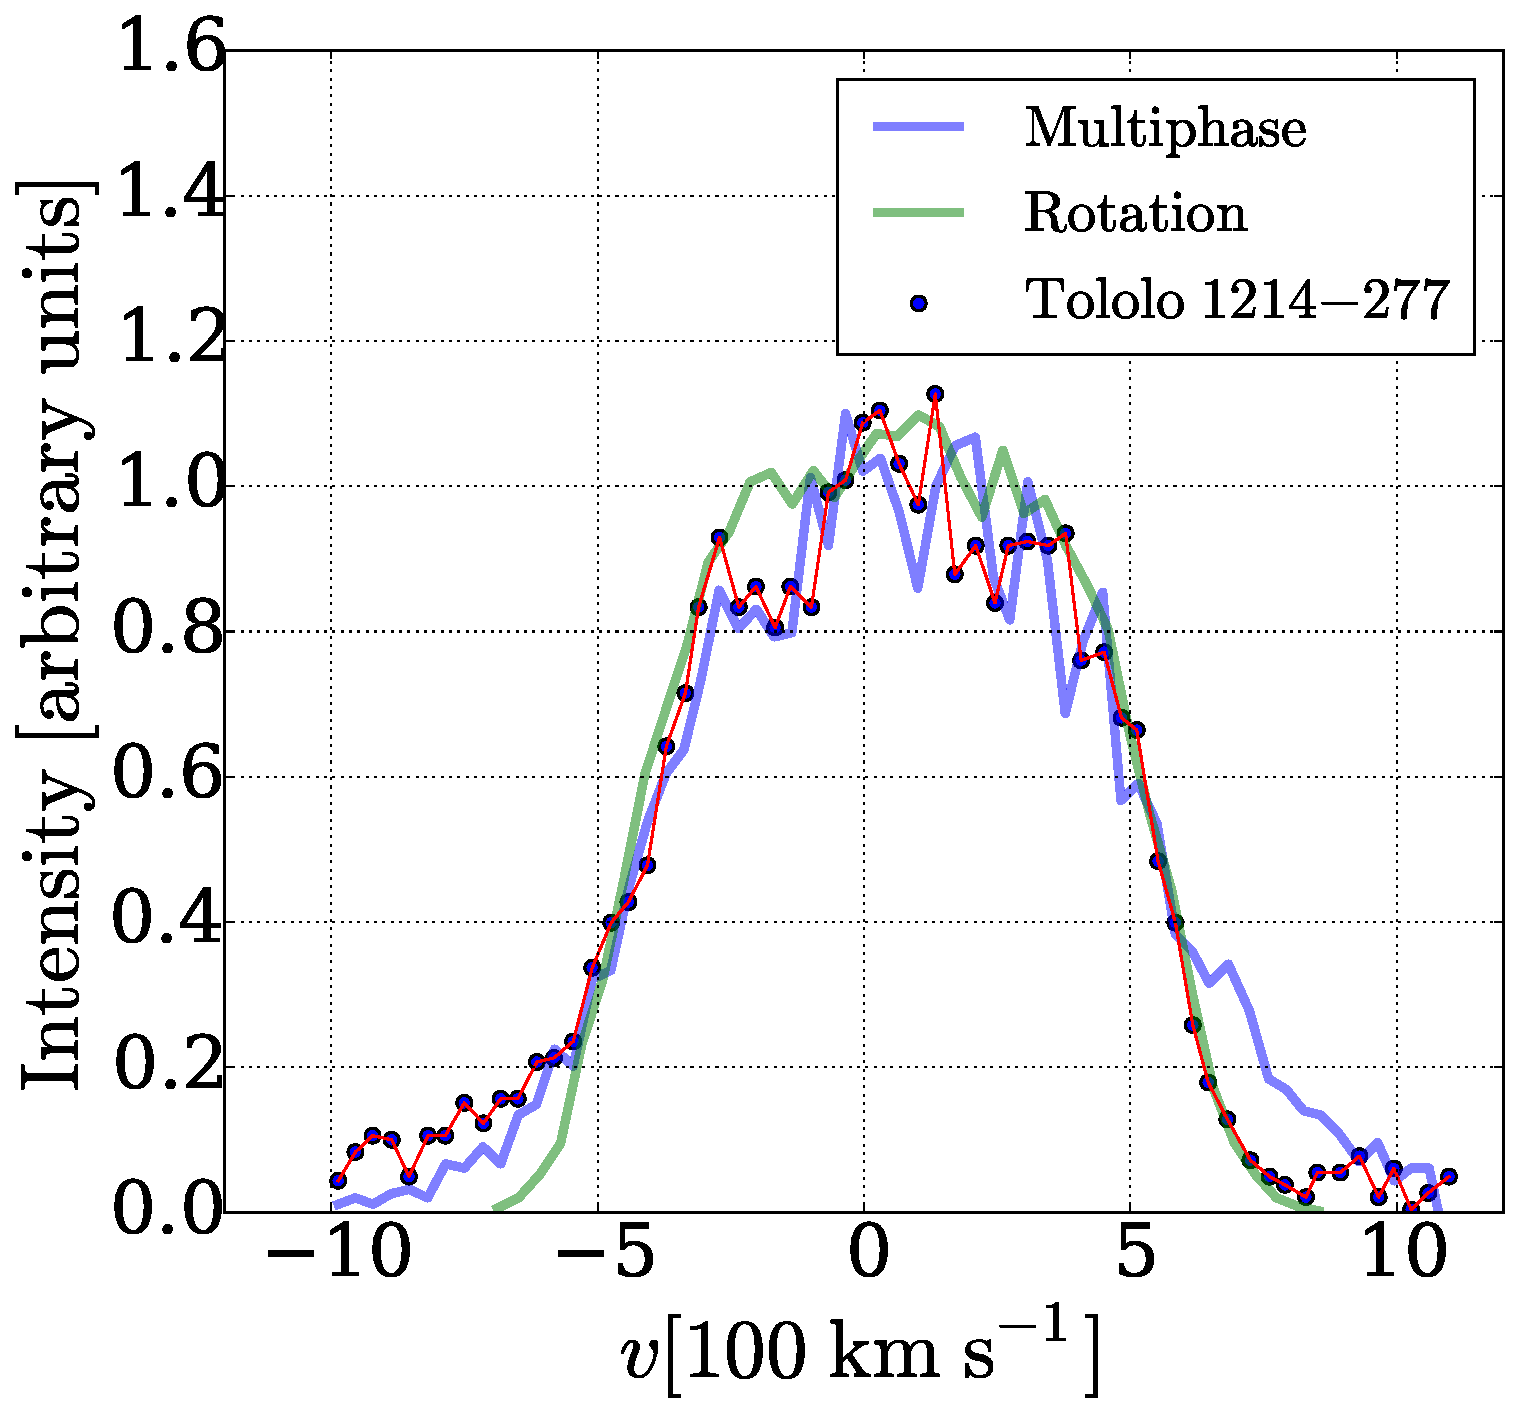
\includegraphics[width=0.8\textwidth]{CLARA-TOL-main.pdf}
\caption{{\bf Broad, single peaked and symmetric Ly-$\alpha$ emission of \tol.}
  Dots correspond to the observational data. The line shows the results
of our best model from a full radiative transfer simulation both for
the rotation and multiphase models.} 
\end{center}
\end{figure}

\bibliography{references}{}
\bibliographystyle{plain}

\newpage 

\section*{\tol\ characteristics}


\begin{table}
\begin{center}
\begin{tabular}{lc}
$\alpha$(2000)$^{a}$ & 12h17min17.1s\\
$\delta$(2000)$^{b}$ & -28d02m32s\\
$l$, $b$ (deg) & 294, 34\\
$m_V$ & 17.5\\
  M$_V$ & -17.6\\ 
$v$(km s$^{-1}$) & 7795\\
Ly-$\alpha$ (erg cm$^{-2}$ s$^{-1}$ \AA$^{-1}$)& $8.1\times 10^{-14}$ \\
Ly-$\alpha$ EW & $70$\AA\\
H$\beta$ (erg cm$^{-2}$ s$^{-1}$ \AA$^{-1}$) & $1.62\times 10^{-14}$ \\
$21$cm (Jy km s$^{-1}$)& $<0.10$ \\
\end{tabular}
\end{center}
\caption{Basic observational characteristics of TOL1214-277
  \cite{Thuan97}\\} 
\end{table}


%\url{http://vizier.u-strasbg.fr/cgi-bin/VizieR?-source=B/2mass}
% TOLOLO 00021
%https://ned.ipac.caltech.edu/cgi-bin/objsearch?objname=Tol+21&extend=no&hconst=73&omegam=0.27&omegav=0.73&corr_z=1&out_csys=Equatorial&out_equinox=J2000.0&obj_sort=RA+or+Longitude&of=pre_text&zv_breaker=30000.0&list_limit=5&img_stamp=YES 
\tol receding velocity is $7785\pm 50$km s$^{-1}$, which translates
into a distance of $106.6$ Mpc (with the Hubble constant $H_{0}$=73
Mpc km s$^{-1}$) 
Its metallicity is $\sim Z_{\odot}/24$ \cite{Izotov04} as derived from optical
spectroscopy. 


The observed flux for the Lyman alpha line is $\sim
8.1\times 10^{-14}$ erg cm$^{-2}$ s$^{-1}$ \cite{Thuan97}
and a Equivalent Width of $70$\AA and its H$\beta$ flux is 
$1.62\times 10^{-14}$ erg cm$^{-2}$ s$^{-1}$ \AA${-1}$
\cite{Izotov04} which gives a Ly$\alpha$/H$\beta$ flux ratio of
4.9$\pm$0.1. The Ly-$\alpha$ flux values correspond to luminosities of
$L_{Ly\alpha}=2.2\times 10^{42}$ erg s$^{-1}$ over a $20$\AA
bandwidth, which in turns translates  into a star formation rate of
$2.0$ M$_{\odot}$ yr$^{-1}$ using a standard conversion factor between
luminosity and star formation rate of $9.1\times 10^{-43}$
$L_{Ly\alpha}$ M$_{\odot}$ yr$^{-1}$. 
The absolute magnitude in the $V$ band translates into a luminosity of
$8.9\times 10^{8}$ L$_{\odot}$.
% using http://tomdwelly.com/tools_fluxtolum.php
Comparing this ratio with the theoretical expectation from case B
recombination of $23.3$ \cite{Hummer1987} one can estimate an escape
fraction of $20$\% for Ly$\alpha$ radiation.
The bolometric UV luminosity is $9.43\pm1.94 \times 10^{8}$
L$_{\odot}$ as measured by GALEX. 

The optical emission  comes from a   region with approximate diameter
4 kpc \cite{Fricke01}. 

There is an upper limit for the  
integrated flux of $<0.10$ Jy km s$^{-1}$, which translates into a
upper limit for the HI mass of $M<2.65\times 10^{8}$ M$_{\odot}$
\cite{pustilnikmartin07}.  

The near-infrared fluxes at $3.6$ $\mu$m and $4.5$ $\mu$m are
$7.71\pm0.55\times 10^{-5}$ Jy and $7.98\pm0.71\times 10^{-5}$ Jy
\cite{2008ApJ...678..804E}.  Using a convertion betwen fluxes and
stellar mass calibrted on the Large Magellanic Cloud $M_{\star} =
10^{5.65} \times F_{3.6}^{2.85} \times F_{4.5}^{-1.85} \times
(D/0.05)^2 M_{\odot}$, where fluxes are in Jy and $D$ is the luminosity
distance to the source in Mpc, we find $M_{\star} = 1.45\pm0.45\times 10^{8}
M_{\odot}$, with a $30\%$ uncertainty coming from the callibration
process \cite{2012AJ....143..139E}.  



\section*{The Rotation Model}

The rotation model corresponds to the work presented in
\cite{GaravitoCamargo2014}. 
In that model the Ly-$\alpha$ photons are propagated 
within a spherical and homogeneous cloud of HI gas undergoing solid
body rotation.
The sphere is fully characterized by three parameters: the optical
depth $\tau$ measured from the center to its surface, the HI
temperature $T$, and the linear surface velocity $V_{\rm max}$.  
Photons are emitted at their natural frequency from the center of the
sphere. 
Including the effect of dust only changes the overall line
normalization but not its shape.  
The results we report in the main body of the paper do not include any
dust model.
In the current work, the radiative transfer simulations were done
using Monte Carlo simulations with the code \texttt{CLARA}
\cite{CLARA}.  

The first important effect of rotation is that it breaks the spherical
symmetry of the static case. 
Now the line's observed morphology depends on the angle $\theta$ between the
line-of-sight (LOS) and the rotation axis. 
LOS parallel to the rotation axis tend to observed the line without
any modification from rotation, while the perpendicular LOS will
observe a maximal change in the line's morphology due to rotation.

The main change in the line's morphology is that it broadens and the
intensity at the center increases. 
For high enough rotational velocities the intensity at the peak's
center increases so much that the line goes from double to single
peaked, sometimes slightly triple peaked.
This is the feature that allows this model to fit the observational
features of \tol.

There is a concise analytical description for those features.
This description takes into account how different parts of the
sphere's surface shift in frequency the \lya photons. 
Different shifts in frequency come from different values for the projected
velocity along the LOS. 
As presented in \cite{CLARA}, using the analytical solution for the
\lya\ spectra of a static sphere plus the right frequency shifts
computed from geometrical considerations, one is able to produce an
analytical solution for the rotating sphere that reproduces the main
features found using the full numerical simulation.

The analytical solution for the rotation sphere was the base to
perform the Markov Chain Monte Carlo Calculation using the
\texttt{emcee} implementation.
We explore flat priors on $V_{\rm max}$ $\log_{10}\tau$, $\log_{10} T$ and
$\theta$ using $500$ steps with $24$ walkers for a total of $12000$
points.
The results are summarized in Figure \ref{emceeresults}. 
From this model we find that the fiducial parameters that could
explain the broad features in \tol\ are $V_{\rm max}=348^{+75}_{-48}$
km s$^{-1}$, $\log \tau = 6.96^{+0.26}_{-0.18}$, $\log_{10} T/\mathrm
{K} = 4.27^{+0.11}_{-0.18}$ and  $\theta = 35.78^{+2.13}_{-1.88}$ degrees.


\begin{figure}
\begin{center}
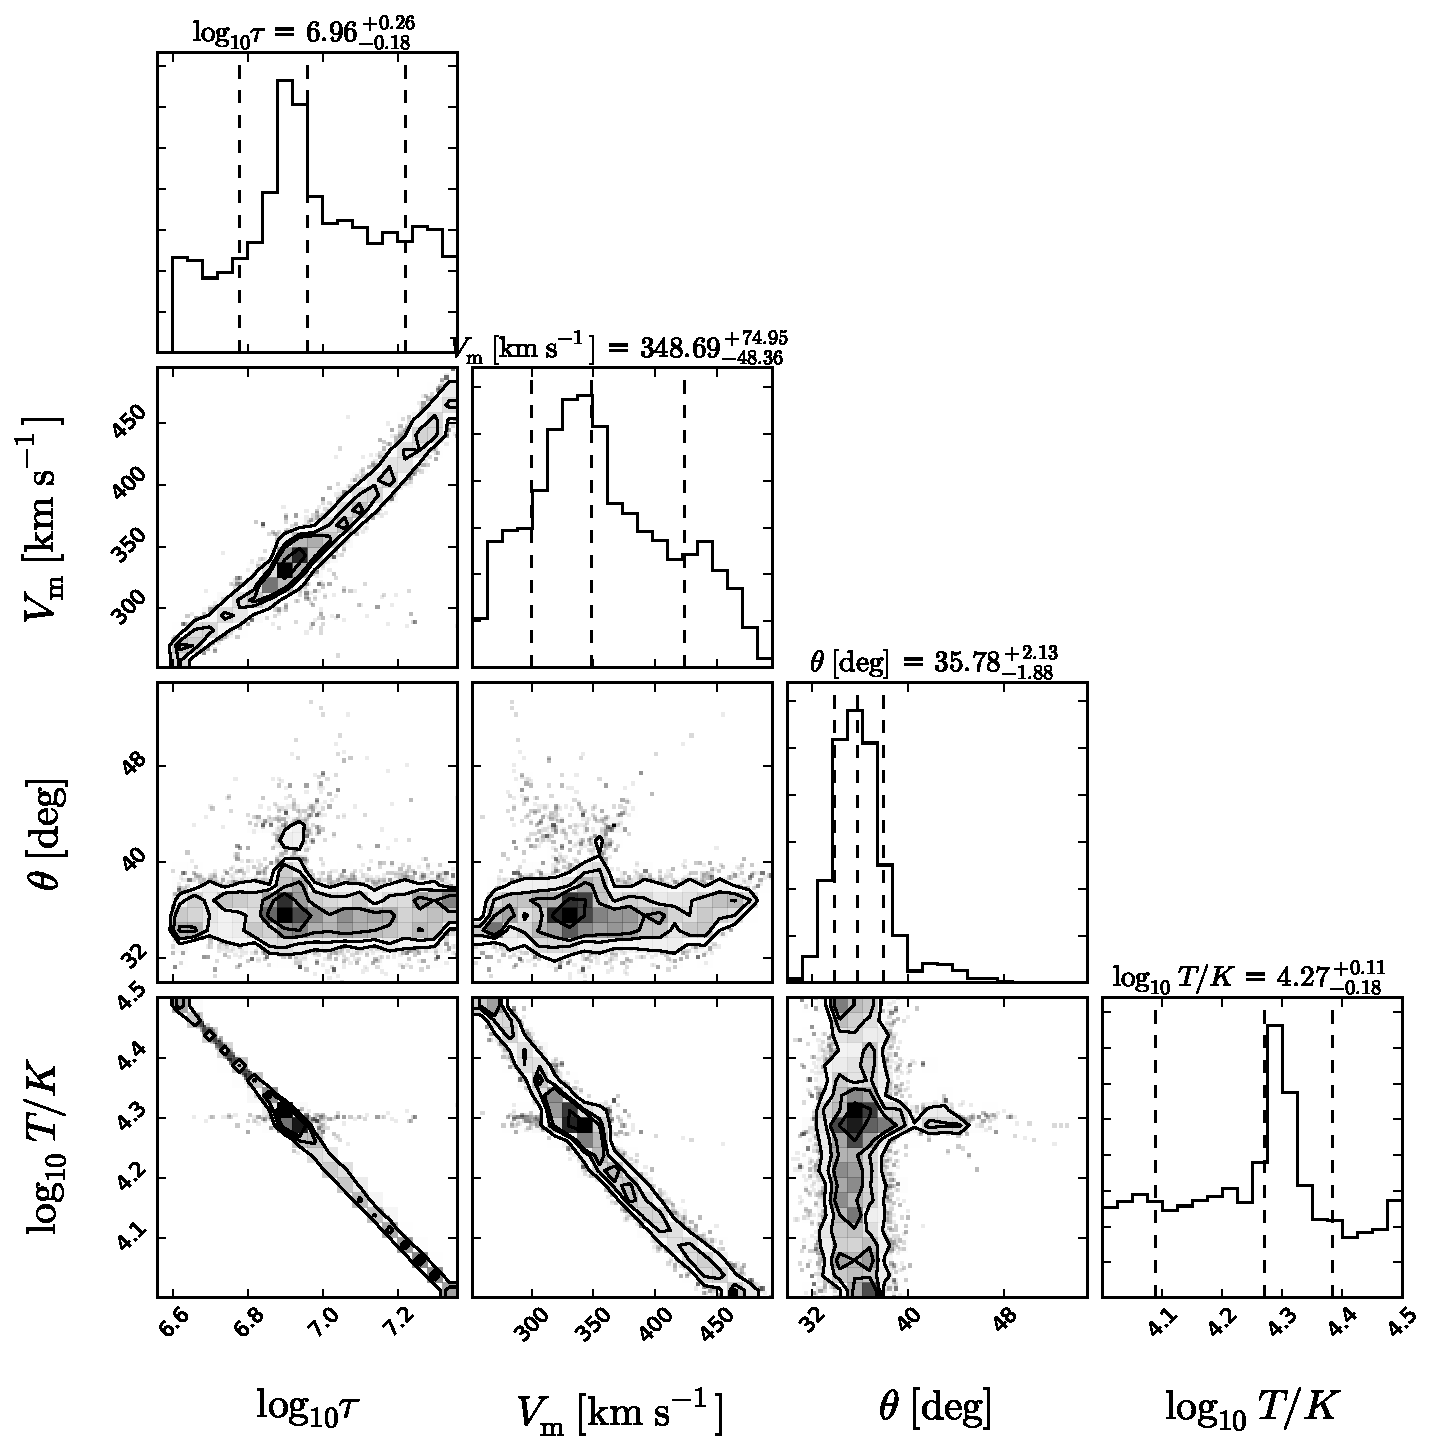
\includegraphics[width=1.0\textwidth]{emcee_results.pdf}
\caption{{\bf Results from the Markov Chain Monte Carlo compuation for
    the rotation model.}\label{emceeresults}} 
\end{center}
\end{figure}


\section*{The Outflow Model}
The galaxy outflow model is a highly sucessful framework to fit
and interprete \lya\ line observations. 



\section*{The Multiphase Model} 

The idealized multiphase model consists of spherical, cold, dens
clumps of neutral hydrogen (and dust) embedded in a hot, ionized
medium. 
The clumps also have a random and an outflowing velocity
component which totals the number of parameters describing the model
to be $14$. 

In order to map out this large parameter space, we randomly drew
$2500$ sets of parameters within a observationally realistic range
(based on the considerations of \cite{Laursen2013ApJ...766..124L})
yielding a large variety of single-, double- and triple-peaked
spectra. 
The full analysis of the the spectral features as well as
more details on the radiative transfer are presented in
\cite{Gronke2016}.    
 
For the current work, we computed the $\chi^2$ for each of the $2500$
Furthermore, we found that some parameters such as the magnitude of
the random clump motion $\sigma_{\rm cl}$ improved the fit
significantly whereas others did not.  

We find that the best constrained parameters are the clump velocity
dispersion $\sigma_{\rm cl}=$\sigmaclump,  the outflowing clump
velocity $v_{\infty {\rm, cl}}=$\inftyclump\ and the probability that
the \lya\ emission comes from the clumps $P_{\rm cl}=$\probaclump.

Qualitatively as \tol\ possesses a very wide spectrum which can be
achieved by subsequent scatterings off (relatively) fast moving clumps
while the multi-phase nature (i.e., the existence of low-density
channels) ensures the high flux at line center as observed.     


\section*{Physical Interpretation}

Both the rotation and the multiphase model constrain the typical
velocity $v$ of the HI gas, with and additional constrain on the typical
size for the emission region $r$ on could estimate a dynamical mass with 

\begin{equation}
M_{\rm dyn} = \frac{v^{2}r}{G} = 1.16\times10^{9}
\left(\frac{v}{100\ \mathrm{km\ s}^{-1}}\right)^2\left(\frac{r}{\mathrm{kpc}}\right) M_{\odot}
\end{equation}

From the multiphase model we obtained $v=$\sigmaclump
and $r=5$ kpc. This corresponds to a dynamical mass of $M_{\rm
  dyn}=2.8^{+1.3}_{-1.2}\times 10^{9}$ $M_{\odot}$ which is at least
$5$ times the HI mass plus the stellar mass estimated from
observations.   

In the rotation model the size of the spherical region, $r_{s}$, can
be infered from the relationship $\tau = \sigma_0 n r_s$, where
$\sigma_0=5.898\times 10^{-14}$cm$^{-2}$ is the Lyman$\alpha$
cross section at the  line's center, $n$ is the number density. 
This expresion can be rewritten as
\begin{equation}
r_{s} = 0.055 \left(\frac{\tau}{10^7}\right) \left(
\frac{\mathrm{atoms\ cm^{-3}}}{n}\right) \mathrm{kpc}.
\end{equation}
%
Using this result and assuming a bound for the number density of
$0.01<n/\mathrm{atoms\ cm^{-3}}<0.1$ we have $0.55
< r_s/\mathrm{kpc}<5.5$.

This is consistent with the  constraint on the total HI mass and the
optical depth $\tau_0$ as we show next. The total HI mass can be
approximated as $M_H = \frac{4\pi}{3} m_H n r_s^3$, where
$m_H=1.67\times 10^{-24}$ gr is the mass of a single Hydrogen atom.
This allows us to write the total hydrogen mass as
\begin{equation}
M_{H} = 5.70 \times 10^{6} \left(\frac{\tau}{10^{7}}\right)
\left(\frac{r_s}{\mathrm{kpc}}\right)^2 M_{\odot}
\end{equation}
%
The uppper limit from the HI mass non-detection imposes $r_{s} <
6.81$ kpc, which is consistent with the bound we found in the first
place, as we wanted to show.

Using those size bounds for the spherical model we find a constrain for
the dynamical mass of $5.45\times 10^{9}M_{\odot} < M_{\rm dyn} <
5.45\times 10^{10} M_{\odot}$. 

\end{document}

